\chapter{Ví dụ minh họa các bước thực hiện}

Ví dụ của chương này là đề số 13, tên ``Ngắn, có quay lui'' trong danh sách đề mẫu của website. Đề có 16 ô trống và đúng một lời giải. Thuật toán cần 79 lần thử, ghi nhận 19 lần và trả lại 3 lần: một lần ở giai đoạn 1, hai lần ở giai đoạn 2. Hai lần ở giai đoạn 2 hợp thành một chuỗi lùi dây chuyền qua hai ô. Toàn bộ 83 bước nằm trong Bảng \ref{tab:illustration-steps} ở cuối chương.

\section{Chọn đề và cách đọc bảng}

Chương này cần một đề đủ ngắn để in trọn từng bước, mà vẫn có quay lui thật. Đề Arto Inkala cần 445.778 lần thử, quá dài. Đề ``Dễ'' chỉ cần 27 lần thử nhưng không quay lui lần nào. Claude viết script \texttt{checks/find\_illustration\_puzzle.py}: xóa ngẫu nhiên 10 đến 16 ô từ một lưới đầy, rồi giữ lại các đề thỏa đúng một lời giải, 50 đến 90 lần thử, 1 đến 3 lần quay lui, có đủ ba kiểu bị loại vì hàng, cột và khối. Trong 12 đề tìm được, Claude chọn đề này vì cả ba lần quay lui nằm gọn trong 35 lần thử đầu, ngay trên hàng 1.

\begin{figure}[H]
  \centering
  \begin{minipage}[t]{0.46\linewidth}
    \centering
    \begingroup\setlength{\tabcolsep}{0pt}\renewcommand{\arraystretch}{1.35}
\begin{tabular}{!{\vrule width 1.2pt}G|G|G!{\vrule width 1.2pt}G|G|G!{\vrule width 1.2pt}G|G|G!{\vrule width 1.2pt}}
\noalign{\hrule height 1.2pt}
\textbf{5} & \textbf{3} & \textbf{4} & \textbf{6} & \textbf{7} &  & \textbf{9} &  &  \\ \hline
\textbf{6} & \textbf{7} &  &  & \textbf{9} & \textbf{5} & \textbf{3} & \textbf{4} & \textbf{8} \\ \hline
 & \textbf{9} & \textbf{8} & \textbf{3} & \textbf{4} &  & \textbf{5} & \textbf{6} & \textbf{7} \\ \noalign{\hrule height 1.2pt}
\textbf{8} &  & \textbf{9} & \textbf{7} & \textbf{6} &  &  & \textbf{2} & \textbf{3} \\ \hline
\textbf{4} &  & \textbf{6} &  & \textbf{5} & \textbf{3} & \textbf{7} & \textbf{9} & \textbf{1} \\ \hline
\textbf{7} & \textbf{1} & \textbf{3} & \textbf{9} &  & \textbf{4} & \textbf{8} & \textbf{5} & \textbf{6} \\ \noalign{\hrule height 1.2pt}
\textbf{9} & \textbf{6} & \textbf{1} & \textbf{5} & \textbf{3} & \textbf{7} & \textbf{2} &  & \textbf{4} \\ \hline
\textbf{2} & \textbf{8} & \textbf{7} & \textbf{4} & \textbf{1} & \textbf{9} & \textbf{6} & \textbf{3} & \textbf{5} \\ \hline
 & \textbf{4} & \textbf{5} &  & \textbf{8} & \textbf{6} & \textbf{1} & \textbf{7} & \textbf{9} \\ \noalign{\hrule height 1.2pt}
\end{tabular}\endgroup

    \par\smallskip\small (a) Đề: 16 ô trống
  \end{minipage}
  \hfill
  \begin{minipage}[t]{0.46\linewidth}
    \centering
    \begingroup\setlength{\tabcolsep}{0pt}\renewcommand{\arraystretch}{1.35}
\begin{tabular}{!{\vrule width 1.2pt}G|G|G!{\vrule width 1.2pt}G|G|G!{\vrule width 1.2pt}G|G|G!{\vrule width 1.2pt}}
\noalign{\hrule height 1.2pt}
\textbf{5} & \textbf{3} & \textbf{4} & \textbf{6} & \textbf{7} & \textcolor{blue!65!black}{8} & \textbf{9} & \textcolor{blue!65!black}{1} & \textcolor{blue!65!black}{2} \\ \hline
\textbf{6} & \textbf{7} & \textcolor{blue!65!black}{2} & \textcolor{blue!65!black}{1} & \textbf{9} & \textbf{5} & \textbf{3} & \textbf{4} & \textbf{8} \\ \hline
\textcolor{blue!65!black}{1} & \textbf{9} & \textbf{8} & \textbf{3} & \textbf{4} & \textcolor{blue!65!black}{2} & \textbf{5} & \textbf{6} & \textbf{7} \\ \noalign{\hrule height 1.2pt}
\textbf{8} & \textcolor{blue!65!black}{5} & \textbf{9} & \textbf{7} & \textbf{6} & \textcolor{blue!65!black}{1} & \textcolor{blue!65!black}{4} & \textbf{2} & \textbf{3} \\ \hline
\textbf{4} & \textcolor{blue!65!black}{2} & \textbf{6} & \textcolor{blue!65!black}{8} & \textbf{5} & \textbf{3} & \textbf{7} & \textbf{9} & \textbf{1} \\ \hline
\textbf{7} & \textbf{1} & \textbf{3} & \textbf{9} & \textcolor{blue!65!black}{2} & \textbf{4} & \textbf{8} & \textbf{5} & \textbf{6} \\ \noalign{\hrule height 1.2pt}
\textbf{9} & \textbf{6} & \textbf{1} & \textbf{5} & \textbf{3} & \textbf{7} & \textbf{2} & \textcolor{blue!65!black}{8} & \textbf{4} \\ \hline
\textbf{2} & \textbf{8} & \textbf{7} & \textbf{4} & \textbf{1} & \textbf{9} & \textbf{6} & \textbf{3} & \textbf{5} \\ \hline
\textcolor{blue!65!black}{3} & \textbf{4} & \textbf{5} & \textcolor{blue!65!black}{2} & \textbf{8} & \textbf{6} & \textbf{1} & \textbf{7} & \textbf{9} \\ \noalign{\hrule height 1.2pt}
\end{tabular}\endgroup

    \par\smallskip\small (b) Lời giải: số in xanh là số thuật toán điền
  \end{minipage}
  \caption{Đề số 13 và lời giải}
  \label{fig:illustration-grids}
\end{figure}

Bảng \ref{tab:illustration-cells} đánh số 16 ô trống theo thứ tự hàng rồi cột. \(S_i\) là số điền vào ô trống thứ \(i\).

\begin{table}[H]
  \centering
  \caption{Vị trí của 16 ô trống}
  \label{tab:illustration-cells}
  \small
  \begin{tabular}{@{}l*{8}{c}@{}}
    \toprule
    \(i\) & 1 & 2 & 3 & 4 & 5 & 6 & 7 & 8 \\
    Ô & (1, 6) & (1, 8) & (1, 9) & (2, 3) & (2, 4) & (3, 1) & (3, 6) & (4, 2) \\
    \midrule
    \(i\) & 9 & 10 & 11 & 12 & 13 & 14 & 15 & 16 \\
    Ô & (4, 6) & (4, 7) & (5, 2) & (5, 4) & (6, 5) & (7, 8) & (9, 1) & (9, 4) \\
    \bottomrule
  \end{tabular}
\end{table}

Trạng thái dữ liệu gồm lưới \texttt{grid}, vectơ \(S\) và ba mảng đánh dấu \texttt{rowUsed}, \texttt{columnUsed}, \texttt{boxUsed} (Chương 4). Mỗi dòng của Bảng \ref{tab:illustration-steps} là một bước thuật toán:

\begin{itemize}
  \item \textbf{Bấm}: số lần bấm nút Từng bước trên trang Giải Sudoku để tới đúng trạng thái đó. Mỗi lần bấm, trang đi một sự kiện, kể cả các sự kiện không có dòng riêng trong bảng như ``ghi nhận'' và ``sang ô kế''. Vì vậy sau mỗi dòng Chấp nhận, cột Bấm tăng 3 (chấp nhận, ghi nhận, sang ô kế). Sau dòng Bị loại hay Trả lại, cột Bấm tăng 1. Ở ô cuối cùng, lần bấm 118 là chấp nhận, lần bấm 119 là ghi nhận, lần bấm 120 là xuất lời giải.
  \item \textbf{Lần thử}, \(i\), \textbf{Ô}, \(j\): bộ đếm lần thử, ô trống thứ mấy, nằm ở đâu, và số đang thử. Dòng Trả lại không tính là một lần thử, nên giữ nguyên bộ đếm của dòng trước, và \(j\) ở dòng đó là số vừa bị xóa.
  \item \textbf{Thao tác} và \textbf{Lý do}: ``Chấp nhận'' là số \(j\) chấp nhận được, thuật toán ghi nhận rồi sang ô trống kế tiếp. ``Bị loại'' kèm hàng, cột hoặc khối bị trùng và ô đang giữ số đó. Số trùng ở nhiều chỗ thì bảng ghi chỗ đầu tiên theo thứ tự hàng, cột, khối, đúng thứ tự thuật toán kiểm tra. ``Trả lại'' là trả lại trạng thái cũ vì ô phía sau đã hết số để thử. ``Có lời giải'' là dòng cuối, không thử thêm số nào, nên bộ đếm lần thử vẫn là 79.
  \item \textbf{\(S\) sau bước}: vectơ \(S_1 \ldots S_{16}\) sau khi bước đó xong, dấu chấm là thành phần chưa có giá trị.
\end{itemize}

Muốn kiểm lại trên website, mở trang Giải Sudoku, chọn ``Đề 13 - Ngắn, có quay lui'' ở ô Đề mẫu, rồi bấm Từng bước. Nút ``Tới lần quay lui kế'' đưa thẳng tới dòng Trả lại kế tiếp, nút ``Lùi một bước'' đi ngược lại. Bộ đếm trên trang cộng dồn từ đầu: 3 ghi nhận nghĩa là thuật toán đã ghi nhận 3 lần, không phải lưới đang có 3 số do thuật toán điền.

\section{Diễn biến}

Hàng 1 đã có các số 5, 3, 4, 6, 7, 9, nên ba ô trống \((1, 6)\), \((1, 8)\), \((1, 9)\) phải nhận đúng ba số 1, 2, 8. Số 8 đã nằm ở ô \((2, 9)\), cùng cột 9 với ô \((1, 9)\) và cùng khối 3 với cả hai ô \((1, 8)\), \((1, 9)\). Vậy chỉ ô \((1, 6)\) nhận được số 8. Người giải bằng tay thấy ngay điều này. Thuật toán thì thử từ nhỏ lên lớn, nên phải đi vào ngõ cụt hai lần mới tới số 8.

\subsection*{Giai đoạn 1: lần thử 1 đến 10, quay lui một ô}

Ở lần thử 1, thuật toán thử số 1 ở ô \((1, 6)\). Hàng 1, cột 6 và khối 2 đều chưa có số 1, nên số 1 chấp nhận được. Thuật toán ghi nhận: \(S_1 = 1\), \texttt{grid[1][6] = 1}, bật \texttt{rowUsed[1][1]}, \texttt{columnUsed[6][1]}, \texttt{boxUsed[2][1]}. Rồi sang ô trống thứ 2.

Ở ô \((1, 8)\), cả 9 số đều trùng. Số 1 trùng ngay với số vừa điền ở ô \((1, 6)\). Số 2 trùng cột 8, số 8 trùng khối 3, các số còn lại trùng hàng 1. Ô \((1, 8)\) hết số, nên sau lần thử 10, ở lần bấm 13, thuật toán trả lại trạng thái cũ của ô \((1, 6)\): xóa số 1 khỏi lưới, tắt ba cờ vừa bật, \(S_1\) trở về trống (Hình \ref{fig:press-13}).

\begin{figure}[H]
  \centering
  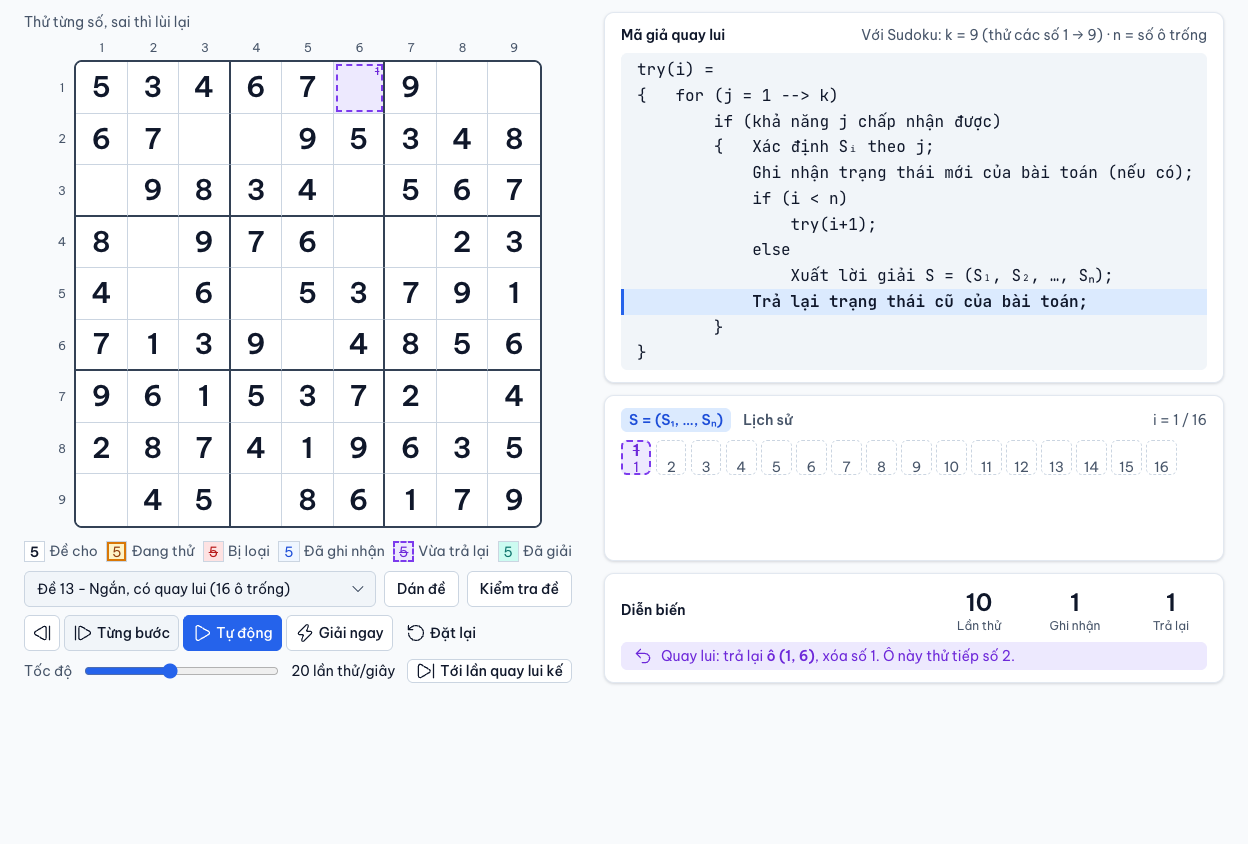
\includegraphics[width=0.95\linewidth]{figures/illustration-press-13.png}
  \caption{Lần bấm 13: thuật toán vừa trả lại ô (1, 6), xóa số 1. Bộ đếm: 10 lần thử, 1 ghi nhận, 1 trả lại}
  \label{fig:press-13}
\end{figure}

\subsection*{Giai đoạn 2: lần thử 11 đến 29, quay lui dây chuyền}

Thuật toán thử tiếp số 2 ở ô \((1, 6)\), và số 2 chấp nhận được (lần thử 11). Lần này ô \((1, 8)\) nhận được số 1, vì số 1 không còn ở hàng 1 nữa (lần thử 12). Ở ô trống thứ 3, ô \((1, 9)\), cả 9 số đều trùng: số 1 trùng với ô \((1, 8)\) vừa điền, số 2 trùng với ô \((1, 6)\), số 8 trùng cột 9, các số còn lại trùng hàng 1. Sau lần thử 21, ở lần bấm 29, thuật toán trả lại ô \((1, 8)\), xóa số 1 (Hình \ref{fig:press-29}).

\begin{figure}[H]
  \centering
  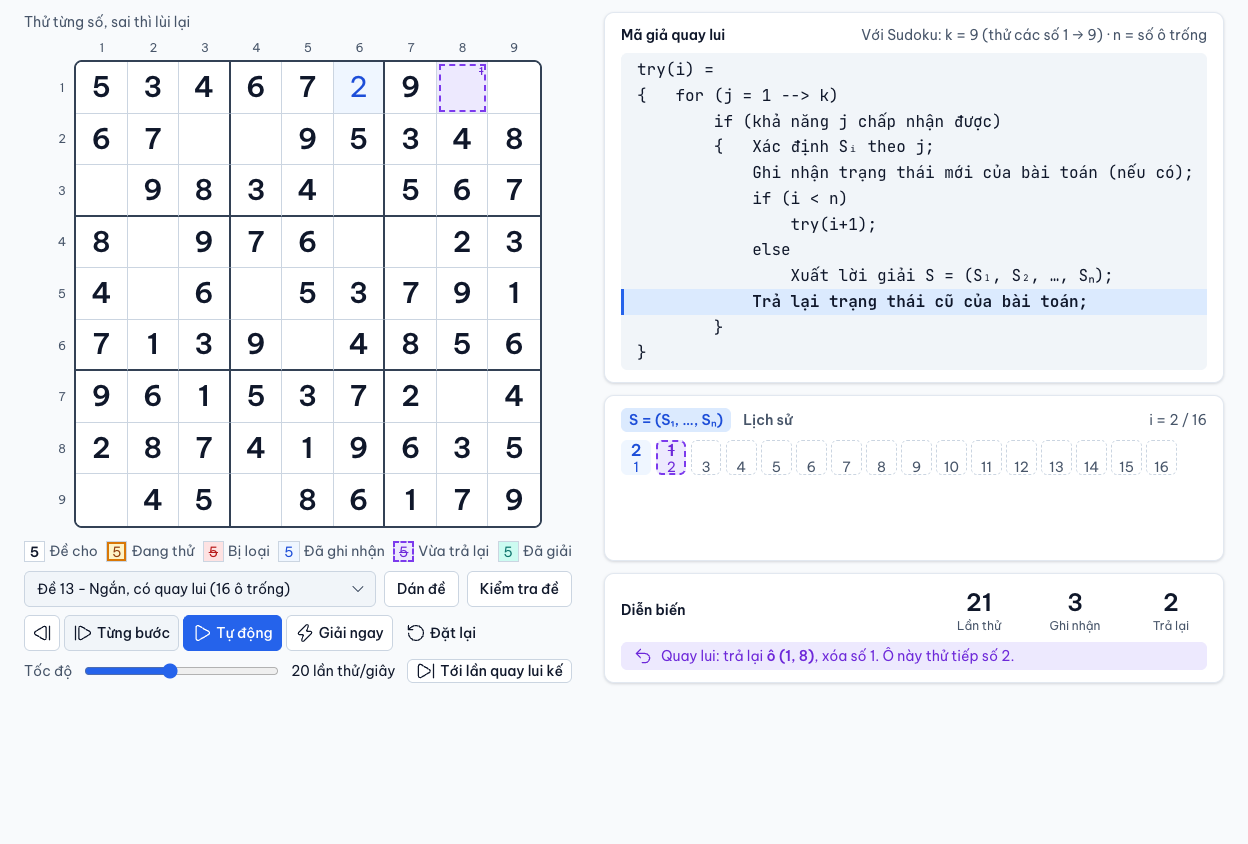
\includegraphics[width=0.95\linewidth]{figures/illustration-press-29.png}
  \caption{Lần bấm 29: thuật toán vừa trả lại ô (1, 8), xóa số 1. Bộ đếm: 21 lần thử, 3 ghi nhận, 2 trả lại}
  \label{fig:press-29}
\end{figure}

Ô \((1, 8)\) chưa hết số, nên thuật toán thử tiếp từ số 2. Số 2 trùng ô \((1, 6)\), số 8 trùng khối 3, các số còn lại trùng hàng 1. Ô \((1, 8)\) hết số lần thứ hai, nên sau lần thử 29, ở lần bấm 38, thuật toán lùi tiếp thêm một ô: trả lại ô \((1, 6)\), xóa số 2 (Hình \ref{fig:press-38}). Hình này gần giống Hình \ref{fig:press-13}. Chỗ khác là số bị gạch trong ô \(S_1\), nay là số 2, và bộ đếm. Đây là quay lui dây chuyền: ô \((1, 9)\) hết số làm ô \((1, 8)\) phải đổi số, và ô \((1, 8)\) hết số làm ô \((1, 6)\) phải đổi số.

\begin{figure}[H]
  \centering
  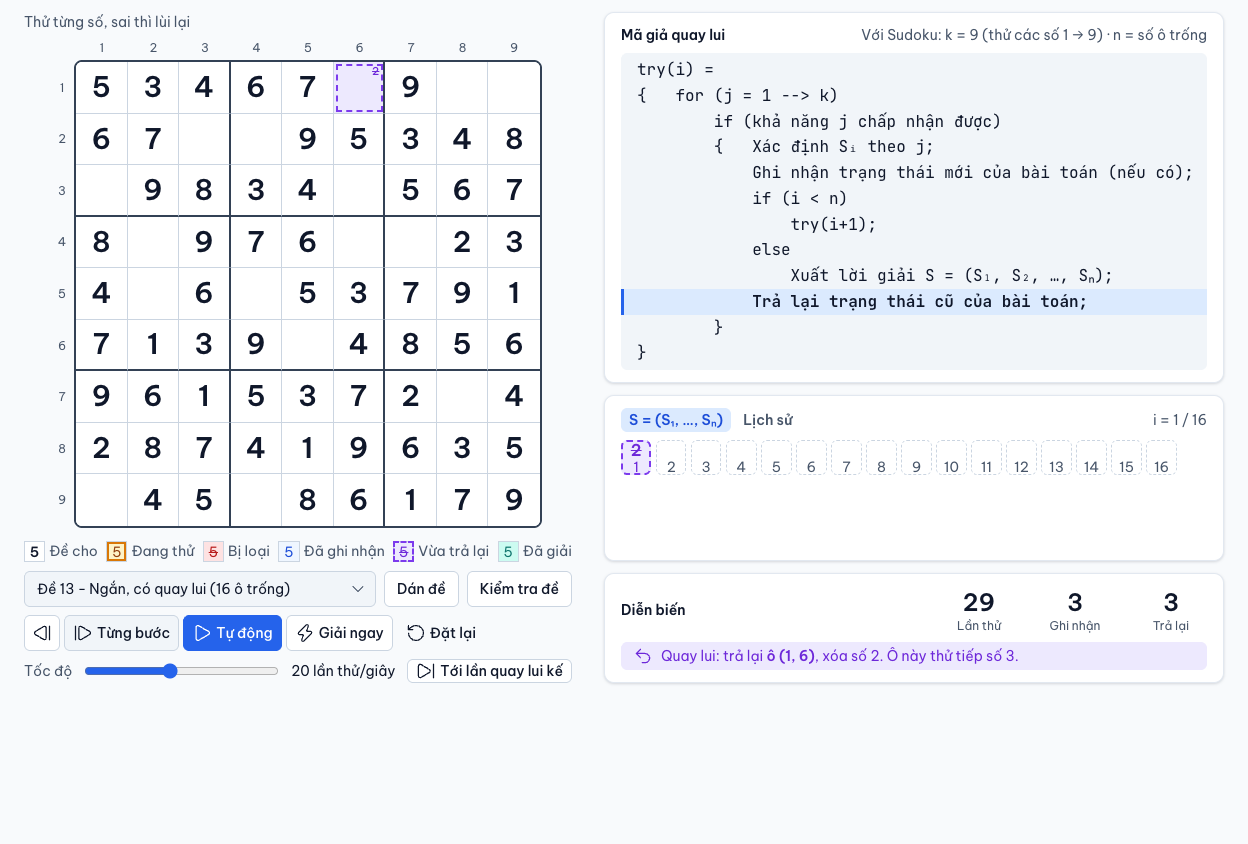
\includegraphics[width=0.95\linewidth]{figures/illustration-press-38.png}
  \caption{Lần bấm 38: thuật toán vừa trả lại ô (1, 6), xóa số 2. Bộ đếm: 29 lần thử, 3 ghi nhận, 3 trả lại}
  \label{fig:press-38}
\end{figure}

\subsection*{Giai đoạn 3: lần thử 30 đến 79, đi thẳng tới lời giải}

Ở ô \((1, 6)\), các số 3 đến 7 đều trùng hàng 1. Số 8 chấp nhận được ở lần thử 35. Từ đây thuật toán không quay lui lần nào nữa. Ô \((1, 8)\) nhận số 1, ô \((1, 9)\) nhận số 2, rồi 13 ô còn lại lần lượt nhận số. Ở lần thử 79 (lần bấm 118), ô trống cuối cùng \((9, 4)\) nhận số 2, và ở lần bấm 120 thuật toán xuất lời giải (Hình \ref{fig:press-120}).

\begin{figure}[H]
  \centering
  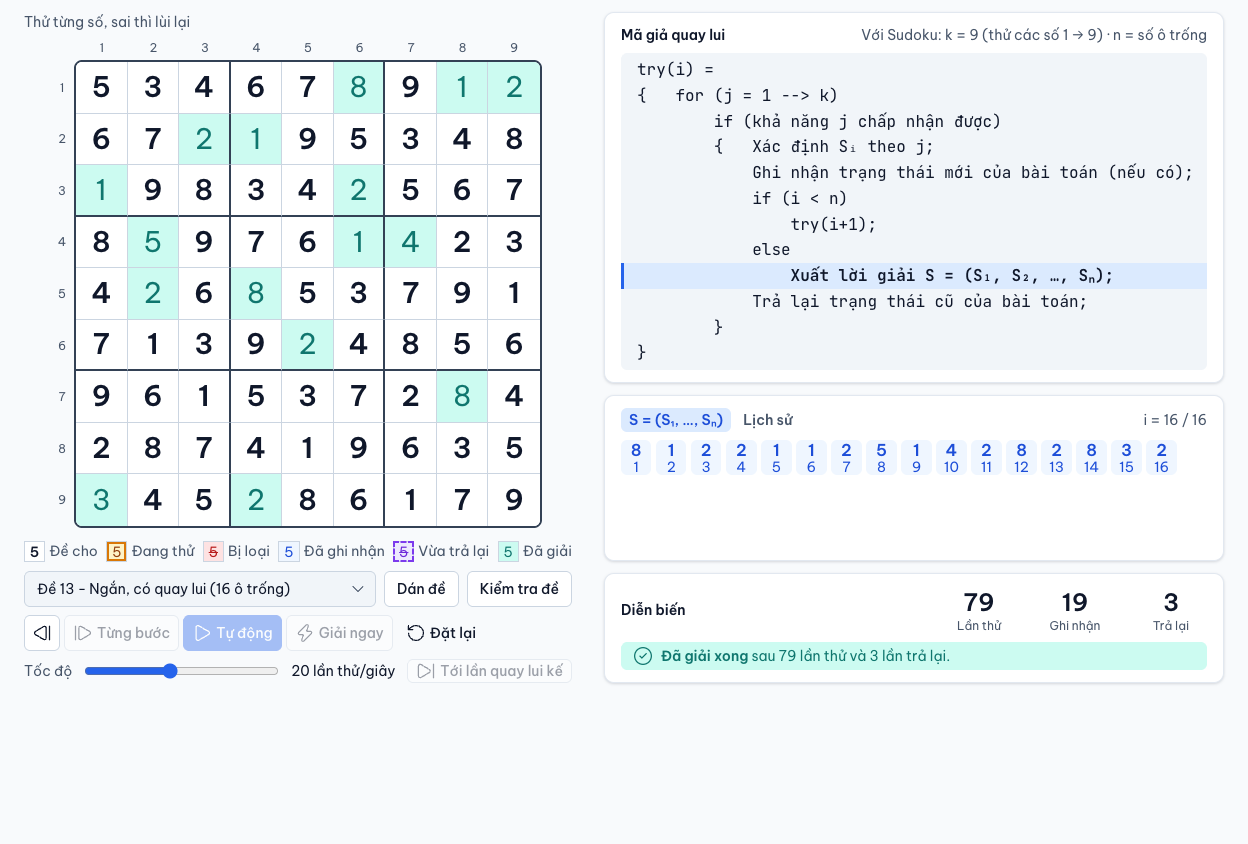
\includegraphics[width=0.95\linewidth]{figures/illustration-press-120.png}
  \caption{Lần bấm 120: đã giải xong. Bộ đếm: 79 lần thử, 19 ghi nhận, 3 trả lại}
  \label{fig:press-120}
\end{figure}

Kết quả cuối cùng là lời giải ở Hình \ref{fig:illustration-grids}(b), với \(S = (8, 1, 2, 2, 1, 1, 2, 5, 1, 4, 2, 8, 2, 8, 3, 2)\). Nếu không phải lùi lần nào, thuật toán chỉ cần thử \(S_1 + S_2 + \cdots + S_{16} = 52\) lần, vì ô thứ \(i\) thử từ 1 tới \(S_i\). Thực tế cần 79 lần, nên ba lần quay lui làm mất 27 lần thử, khoảng một phần ba tổng số. Thuật toán thử theo thứ tự cố định nên không ``nhìn'' trước như người giải bằng tay. Với cùng đề này, cách điền ô ít khả năng nhất trước (mục \ref{sec:variants}) chỉ cần 52 lần thử và không quay lui lần nào.

\section{Ví dụ thứ hai: quay lui qua sáu ô}
\label{sec:deep-example}

Ví dụ trên chỉ quay lui ở hàng 1. Đề mẫu số 3 ``Vừa'' có 40 ô trống, cần 1.909 lần thử và 187 lần trả lại, nên cho thấy một lần quay lui sâu hơn nhiều. Bảng \ref{tab:excerpt-steps} ghi các bước từ lần thử 783 đến lần thử 816, tức lần bấm 1.044 đến 1.089. Cột \(S_{13} \ldots S_{19}\) chỉ giữ bảy thành phần của vectơ \(S\) đang thay đổi trong đoạn này, vì đề có tới 40 thành phần.

Ở lần thử 704, thuật toán điền số 8 vào ô \((4, 1)\), tức \(S_{13} = 8\). Nhánh phía sau còn sống thêm 99 lần thử mới chết hẳn. Ở lần thử 783, ô \((5, 2)\) (\(i = 19\)) hết số: cả 9 số đều trùng. Từ đây thuật toán lùi liên tiếp qua sáu ô:

\begin{itemize}
  \item Ô \((5, 1)\) đang giữ 4. Các số 5 đến 9 đều trùng (lần thử 784 đến 788), nên thuật toán trả lại ô này.
  \item Ô \((4, 9)\) đang giữ 3. Các số 4 đến 9 đều trùng (lần thử 789 đến 794), nên trả lại tiếp.
  \item Ô \((4, 7)\) đang giữ 4. Các số 5 đến 9 đều trùng (lần thử 795 đến 799), nên trả lại tiếp.
  \item Ô \((4, 3)\) đang giữ 9, số cuối cùng, nên không còn số nào để thử. Thuật toán trả lại ngay, không tốn lần thử nào.
  \item Ô \((4, 2)\) đang giữ 5. Các số 6 đến 9 đều trùng (lần thử 800 đến 803), nên trả lại tiếp.
  \item Ô \((4, 1)\) đang giữ 8, số điền ở lần thử 704. Ở lần thử 803, thuật toán trả lại ô \((4, 1)\) (Hình \ref{fig:press-1070}) và thử tiếp số 9, được chấp nhận ở lần thử 804.
\end{itemize}

Sau đó thuật toán điền lại các ô phía sau. Ô \((4, 2)\) loại các số 1 đến 4 rồi nhận số 5 (lần thử 809). Ô \((4, 3)\) loại số 1 và 2 rồi nhận số 3 (lần thử 812). Ô \((4, 7)\) loại các số 1, 2 và 3 rồi nhận số 4 (lần thử 816). Số 8 mà ô \((4, 1)\) nhận ở lần thử 704 cũng nằm trong lời giải đầu tiên thuật toán tìm ra. Nhánh của nó chết vì trong các ô \(S_4\) đến \(S_{12}\) phía trước còn ô mang số khác với lời giải đó (\(S_4 = 2\) thay vì 7). Số 8 chỉ được điền lại ở lần thử 1.253, sau khi các ô đó đã đổi.

\begin{figure}[H]
  \centering
  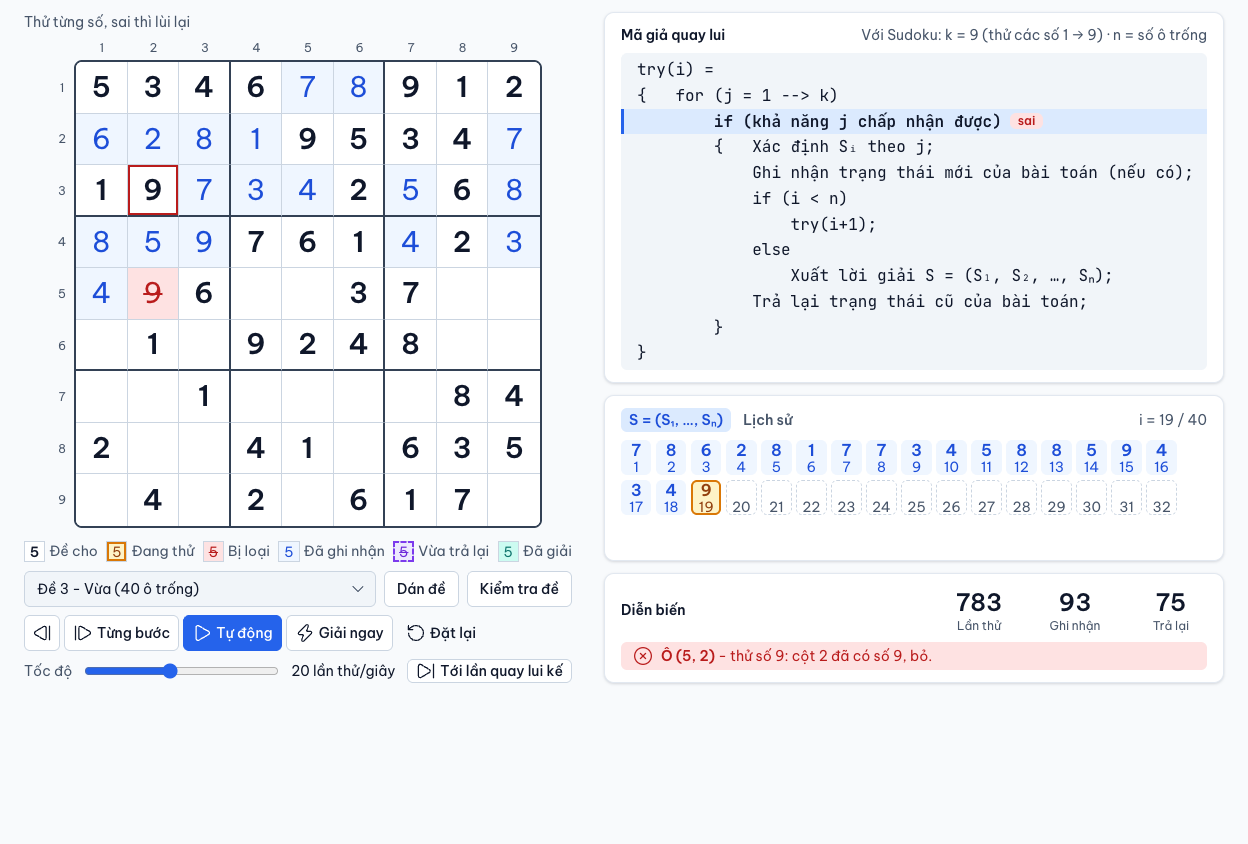
\includegraphics[width=0.85\linewidth]{figures/excerpt-press-1044.png}
  \caption{Lần bấm 1.044: ô \((5, 2)\) vừa hết số ở lần thử 783. Bộ đếm: 783 lần thử, 93 ghi nhận, 75 trả lại}
  \label{fig:press-1044}
\end{figure}

\begin{figure}[H]
  \centering
  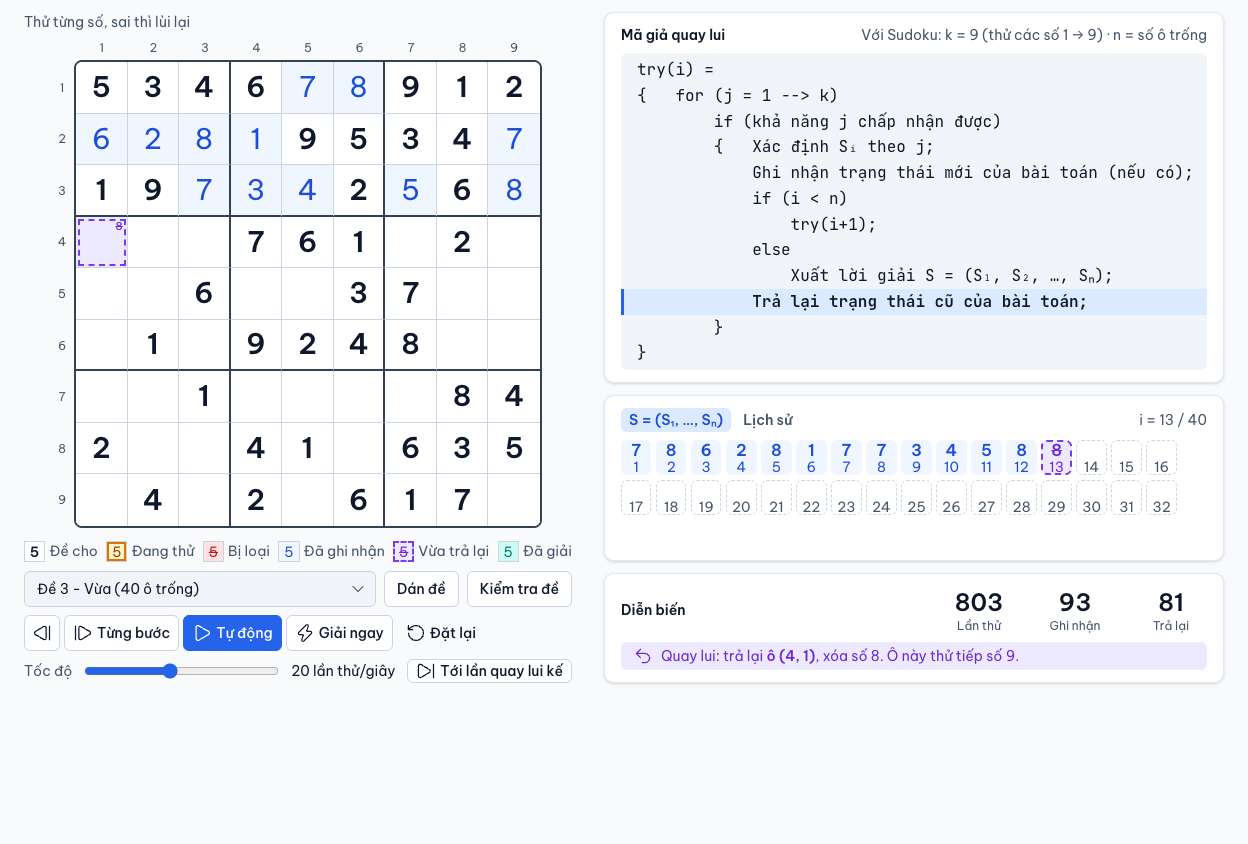
\includegraphics[width=0.85\linewidth]{figures/excerpt-press-1070.png}
  \caption{Lần bấm 1.070: thuật toán vừa trả lại ô \((4, 1)\), xóa số 8. Bộ đếm: 803 lần thử, 93 ghi nhận, 81 trả lại}
  \label{fig:press-1070}
\end{figure}

\begin{figure}[H]
  \centering
  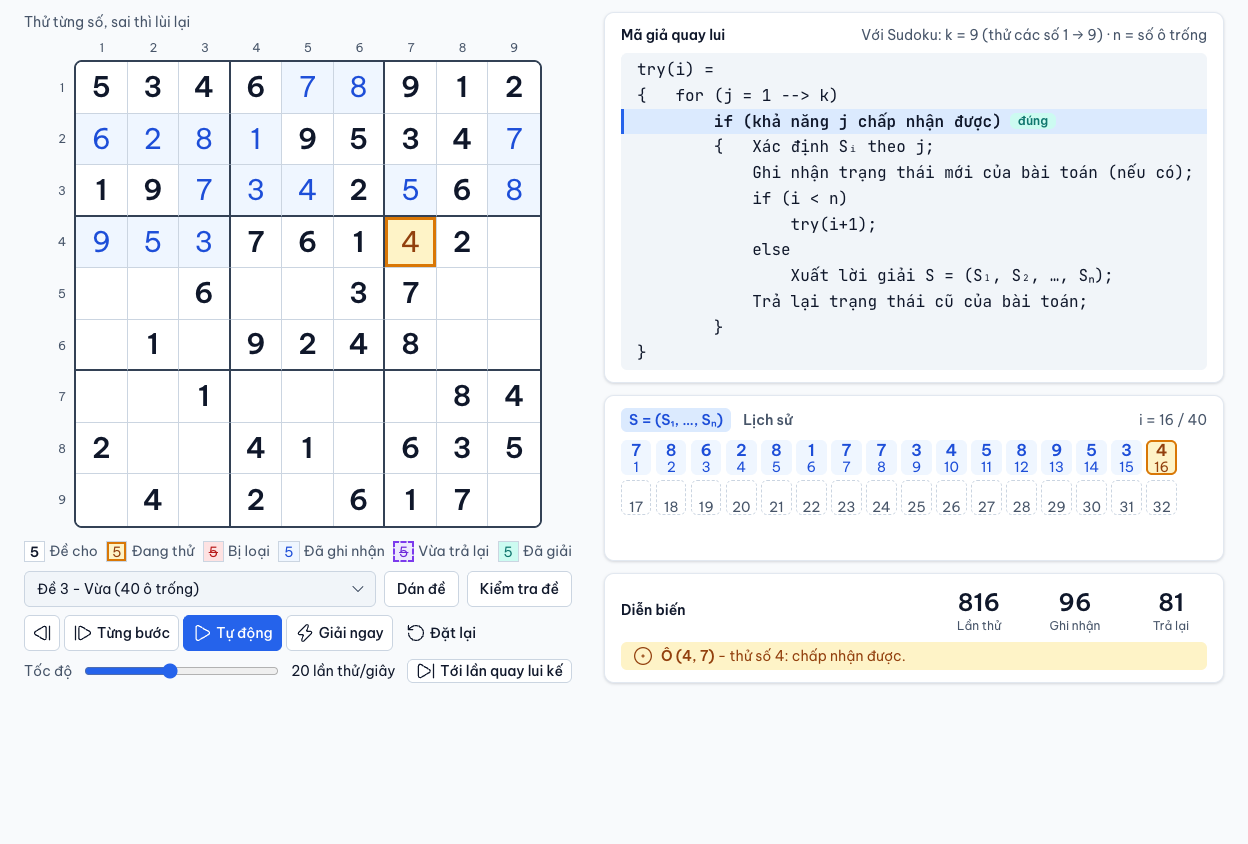
\includegraphics[width=0.85\linewidth]{figures/excerpt-press-1089.png}
  \caption{Lần bấm 1.089: ô \((4, 7)\) vừa nhận số 4 ở lần thử 816. Bộ đếm: 816 lần thử, 96 ghi nhận, 81 trả lại}
  \label{fig:press-1089}
\end{figure}

Muốn kiểm lại trên website, chọn đề 3 ``Vừa'' ở trang Giải Sudoku rồi bấm Từng bước đủ số lần ở cột Bấm. Nút ``Tới lần quay lui kế'' cho nhảy qua từng lần trả lại thay cho việc bấm tay hàng nghìn lần.

\begingroup\footnotesize\setlength{\tabcolsep}{3pt}
\begin{longtable}{@{}rrrcc>{\raggedright\arraybackslash}p{2.1cm}>{\raggedright\arraybackslash}p{3.7cm}>{\ttfamily}l@{}}
\caption{Các bước từ lần thử 783 đến lần thử 816 của đề ``Vừa''}\label{tab:excerpt-steps}\\
\toprule
\textbf{Bấm} & \textbf{Lần thử} & \(\boldsymbol{i}\) & \textbf{Ô} & \(\boldsymbol{j}\) & \textbf{Thao tác} & \textbf{Lý do} & \multicolumn{1}{l}{\textbf{\(S_{13} \ldots S_{19}\) sau bước}} \\
\midrule
\endfirsthead
\toprule
\textbf{Bấm} & \textbf{Lần thử} & \(\boldsymbol{i}\) & \textbf{Ô} & \(\boldsymbol{j}\) & \textbf{Thao tác} & \textbf{Lý do} & \multicolumn{1}{l}{\textbf{\(S_{13} \ldots S_{19}\) sau bước}} \\
\midrule
\endhead
\bottomrule
\endfoot
1044 & 783 & 19 & (5, 2) & 9 & Bị loại & trùng cột 2 ở ô (3, 2) & 8 5 9 4 3 4 . \\
1045 & 783 & 18 & (5, 1) & 4 & Trả lại & ô sau hết số & 8 5 9 4 3 . . \\
1046 & 784 & 18 & (5, 1) & 5 & Bị loại & trùng cột 1 ở ô (1, 1) & 8 5 9 4 3 . . \\
1047 & 785 & 18 & (5, 1) & 6 & Bị loại & trùng hàng 5 ở ô (5, 3) & 8 5 9 4 3 . . \\
1048 & 786 & 18 & (5, 1) & 7 & Bị loại & trùng hàng 5 ở ô (5, 7) & 8 5 9 4 3 . . \\
1049 & 787 & 18 & (5, 1) & 8 & Bị loại & trùng cột 1 ở ô (4, 1) & 8 5 9 4 3 . . \\
1050 & 788 & 18 & (5, 1) & 9 & Bị loại & trùng khối 4 ở ô (4, 3) & 8 5 9 4 3 . . \\
1051 & 788 & 17 & (4, 9) & 3 & Trả lại & ô sau hết số & 8 5 9 4 . . . \\
1052 & 789 & 17 & (4, 9) & 4 & Bị loại & trùng hàng 4 ở ô (4, 7) & 8 5 9 4 . . . \\
1053 & 790 & 17 & (4, 9) & 5 & Bị loại & trùng hàng 4 ở ô (4, 2) & 8 5 9 4 . . . \\
1054 & 791 & 17 & (4, 9) & 6 & Bị loại & trùng hàng 4 ở ô (4, 5) & 8 5 9 4 . . . \\
1055 & 792 & 17 & (4, 9) & 7 & Bị loại & trùng hàng 4 ở ô (4, 4) & 8 5 9 4 . . . \\
1056 & 793 & 17 & (4, 9) & 8 & Bị loại & trùng hàng 4 ở ô (4, 1) & 8 5 9 4 . . . \\
1057 & 794 & 17 & (4, 9) & 9 & Bị loại & trùng hàng 4 ở ô (4, 3) & 8 5 9 4 . . . \\
1058 & 794 & 16 & (4, 7) & 4 & Trả lại & ô sau hết số & 8 5 9 . . . . \\
1059 & 795 & 16 & (4, 7) & 5 & Bị loại & trùng hàng 4 ở ô (4, 2) & 8 5 9 . . . . \\
1060 & 796 & 16 & (4, 7) & 6 & Bị loại & trùng hàng 4 ở ô (4, 5) & 8 5 9 . . . . \\
1061 & 797 & 16 & (4, 7) & 7 & Bị loại & trùng hàng 4 ở ô (4, 4) & 8 5 9 . . . . \\
1062 & 798 & 16 & (4, 7) & 8 & Bị loại & trùng hàng 4 ở ô (4, 1) & 8 5 9 . . . . \\
1063 & 799 & 16 & (4, 7) & 9 & Bị loại & trùng hàng 4 ở ô (4, 3) & 8 5 9 . . . . \\
1064 & 799 & 15 & (4, 3) & 9 & Trả lại & ô sau hết số & 8 5 . . . . . \\
1065 & 799 & 14 & (4, 2) & 5 & Trả lại & ô sau hết số & 8 . . . . . . \\
1066 & 800 & 14 & (4, 2) & 6 & Bị loại & trùng hàng 4 ở ô (4, 5) & 8 . . . . . . \\
1067 & 801 & 14 & (4, 2) & 7 & Bị loại & trùng hàng 4 ở ô (4, 4) & 8 . . . . . . \\
1068 & 802 & 14 & (4, 2) & 8 & Bị loại & trùng hàng 4 ở ô (4, 1) & 8 . . . . . . \\
1069 & 803 & 14 & (4, 2) & 9 & Bị loại & trùng cột 2 ở ô (3, 2) & 8 . . . . . . \\
1070 & 803 & 13 & (4, 1) & 8 & Trả lại & ô sau hết số & . . . . . . . \\
1071 & 804 & 13 & (4, 1) & 9 & Chấp nhận & không trùng & 9 . . . . . . \\
1074 & 805 & 14 & (4, 2) & 1 & Bị loại & trùng hàng 4 ở ô (4, 6) & 9 . . . . . . \\
1075 & 806 & 14 & (4, 2) & 2 & Bị loại & trùng hàng 4 ở ô (4, 8) & 9 . . . . . . \\
1076 & 807 & 14 & (4, 2) & 3 & Bị loại & trùng cột 2 ở ô (1, 2) & 9 . . . . . . \\
1077 & 808 & 14 & (4, 2) & 4 & Bị loại & trùng cột 2 ở ô (9, 2) & 9 . . . . . . \\
1078 & 809 & 14 & (4, 2) & 5 & Chấp nhận & không trùng & 9 5 . . . . . \\
1081 & 810 & 15 & (4, 3) & 1 & Bị loại & trùng hàng 4 ở ô (4, 6) & 9 5 . . . . . \\
1082 & 811 & 15 & (4, 3) & 2 & Bị loại & trùng hàng 4 ở ô (4, 8) & 9 5 . . . . . \\
1083 & 812 & 15 & (4, 3) & 3 & Chấp nhận & không trùng & 9 5 3 . . . . \\
1086 & 813 & 16 & (4, 7) & 1 & Bị loại & trùng hàng 4 ở ô (4, 6) & 9 5 3 . . . . \\
1087 & 814 & 16 & (4, 7) & 2 & Bị loại & trùng hàng 4 ở ô (4, 8) & 9 5 3 . . . . \\
1088 & 815 & 16 & (4, 7) & 3 & Bị loại & trùng hàng 4 ở ô (4, 3) & 9 5 3 . . . . \\
1089 & 816 & 16 & (4, 7) & 4 & Chấp nhận & không trùng & 9 5 3 4 . . . \\
\end{longtable}
\endgroup


\section{Bảng toàn bộ các bước}

\begingroup\footnotesize\setlength{\tabcolsep}{3pt}
\begin{longtable}{@{}rrrcc>{\raggedright\arraybackslash}p{2.1cm}>{\raggedright\arraybackslash}p{3.3cm}>{\ttfamily}l@{}}
\caption{Toàn bộ các bước giải đề số 13}\label{tab:illustration-steps}\\
\toprule
\textbf{Bấm} & \textbf{Lần thử} & \(\boldsymbol{i}\) & \textbf{Ô} & \(\boldsymbol{j}\) & \textbf{Thao tác} & \textbf{Lý do} & \multicolumn{1}{l}{\textbf{\(S\) sau bước}} \\
\midrule
\endfirsthead
\toprule
\textbf{Bấm} & \textbf{Lần thử} & \(\boldsymbol{i}\) & \textbf{Ô} & \(\boldsymbol{j}\) & \textbf{Thao tác} & \textbf{Lý do} & \multicolumn{1}{l}{\textbf{\(S\) sau bước}} \\
\midrule
\endhead
\bottomrule
\endfoot
1 & 1 & 1 & (1, 6) & 1 & Chấp nhận & không trùng & 1 . . . . . . . . . . . . . . . \\
4 & 2 & 2 & (1, 8) & 1 & Bị loại & trùng hàng 1 ở ô (1, 6) & 1 . . . . . . . . . . . . . . . \\
5 & 3 & 2 & (1, 8) & 2 & Bị loại & trùng cột 8 ở ô (4, 8) & 1 . . . . . . . . . . . . . . . \\
6 & 4 & 2 & (1, 8) & 3 & Bị loại & trùng hàng 1 ở ô (1, 2) & 1 . . . . . . . . . . . . . . . \\
7 & 5 & 2 & (1, 8) & 4 & Bị loại & trùng hàng 1 ở ô (1, 3) & 1 . . . . . . . . . . . . . . . \\
8 & 6 & 2 & (1, 8) & 5 & Bị loại & trùng hàng 1 ở ô (1, 1) & 1 . . . . . . . . . . . . . . . \\
9 & 7 & 2 & (1, 8) & 6 & Bị loại & trùng hàng 1 ở ô (1, 4) & 1 . . . . . . . . . . . . . . . \\
10 & 8 & 2 & (1, 8) & 7 & Bị loại & trùng hàng 1 ở ô (1, 5) & 1 . . . . . . . . . . . . . . . \\
11 & 9 & 2 & (1, 8) & 8 & Bị loại & trùng khối 3 ở ô (2, 9) & 1 . . . . . . . . . . . . . . . \\
12 & 10 & 2 & (1, 8) & 9 & Bị loại & trùng hàng 1 ở ô (1, 7) & 1 . . . . . . . . . . . . . . . \\
13 & 10 & 1 & (1, 6) & 1 & Trả lại & ô sau hết số & . . . . . . . . . . . . . . . . \\
14 & 11 & 1 & (1, 6) & 2 & Chấp nhận & không trùng & 2 . . . . . . . . . . . . . . . \\
17 & 12 & 2 & (1, 8) & 1 & Chấp nhận & không trùng & 2 1 . . . . . . . . . . . . . . \\
20 & 13 & 3 & (1, 9) & 1 & Bị loại & trùng hàng 1 ở ô (1, 8) & 2 1 . . . . . . . . . . . . . . \\
21 & 14 & 3 & (1, 9) & 2 & Bị loại & trùng hàng 1 ở ô (1, 6) & 2 1 . . . . . . . . . . . . . . \\
22 & 15 & 3 & (1, 9) & 3 & Bị loại & trùng hàng 1 ở ô (1, 2) & 2 1 . . . . . . . . . . . . . . \\
23 & 16 & 3 & (1, 9) & 4 & Bị loại & trùng hàng 1 ở ô (1, 3) & 2 1 . . . . . . . . . . . . . . \\
24 & 17 & 3 & (1, 9) & 5 & Bị loại & trùng hàng 1 ở ô (1, 1) & 2 1 . . . . . . . . . . . . . . \\
25 & 18 & 3 & (1, 9) & 6 & Bị loại & trùng hàng 1 ở ô (1, 4) & 2 1 . . . . . . . . . . . . . . \\
26 & 19 & 3 & (1, 9) & 7 & Bị loại & trùng hàng 1 ở ô (1, 5) & 2 1 . . . . . . . . . . . . . . \\
27 & 20 & 3 & (1, 9) & 8 & Bị loại & trùng cột 9 ở ô (2, 9) & 2 1 . . . . . . . . . . . . . . \\
28 & 21 & 3 & (1, 9) & 9 & Bị loại & trùng hàng 1 ở ô (1, 7) & 2 1 . . . . . . . . . . . . . . \\
29 & 21 & 2 & (1, 8) & 1 & Trả lại & ô sau hết số & 2 . . . . . . . . . . . . . . . \\
30 & 22 & 2 & (1, 8) & 2 & Bị loại & trùng hàng 1 ở ô (1, 6) & 2 . . . . . . . . . . . . . . . \\
31 & 23 & 2 & (1, 8) & 3 & Bị loại & trùng hàng 1 ở ô (1, 2) & 2 . . . . . . . . . . . . . . . \\
32 & 24 & 2 & (1, 8) & 4 & Bị loại & trùng hàng 1 ở ô (1, 3) & 2 . . . . . . . . . . . . . . . \\
33 & 25 & 2 & (1, 8) & 5 & Bị loại & trùng hàng 1 ở ô (1, 1) & 2 . . . . . . . . . . . . . . . \\
34 & 26 & 2 & (1, 8) & 6 & Bị loại & trùng hàng 1 ở ô (1, 4) & 2 . . . . . . . . . . . . . . . \\
35 & 27 & 2 & (1, 8) & 7 & Bị loại & trùng hàng 1 ở ô (1, 5) & 2 . . . . . . . . . . . . . . . \\
36 & 28 & 2 & (1, 8) & 8 & Bị loại & trùng khối 3 ở ô (2, 9) & 2 . . . . . . . . . . . . . . . \\
37 & 29 & 2 & (1, 8) & 9 & Bị loại & trùng hàng 1 ở ô (1, 7) & 2 . . . . . . . . . . . . . . . \\
38 & 29 & 1 & (1, 6) & 2 & Trả lại & ô sau hết số & . . . . . . . . . . . . . . . . \\
39 & 30 & 1 & (1, 6) & 3 & Bị loại & trùng hàng 1 ở ô (1, 2) & . . . . . . . . . . . . . . . . \\
40 & 31 & 1 & (1, 6) & 4 & Bị loại & trùng hàng 1 ở ô (1, 3) & . . . . . . . . . . . . . . . . \\
41 & 32 & 1 & (1, 6) & 5 & Bị loại & trùng hàng 1 ở ô (1, 1) & . . . . . . . . . . . . . . . . \\
42 & 33 & 1 & (1, 6) & 6 & Bị loại & trùng hàng 1 ở ô (1, 4) & . . . . . . . . . . . . . . . . \\
43 & 34 & 1 & (1, 6) & 7 & Bị loại & trùng hàng 1 ở ô (1, 5) & . . . . . . . . . . . . . . . . \\
44 & 35 & 1 & (1, 6) & 8 & Chấp nhận & không trùng & 8 . . . . . . . . . . . . . . . \\
47 & 36 & 2 & (1, 8) & 1 & Chấp nhận & không trùng & 8 1 . . . . . . . . . . . . . . \\
50 & 37 & 3 & (1, 9) & 1 & Bị loại & trùng hàng 1 ở ô (1, 8) & 8 1 . . . . . . . . . . . . . . \\
51 & 38 & 3 & (1, 9) & 2 & Chấp nhận & không trùng & 8 1 2 . . . . . . . . . . . . . \\
54 & 39 & 4 & (2, 3) & 1 & Bị loại & trùng cột 3 ở ô (7, 3) & 8 1 2 . . . . . . . . . . . . . \\
55 & 40 & 4 & (2, 3) & 2 & Chấp nhận & không trùng & 8 1 2 2 . . . . . . . . . . . . \\
58 & 41 & 5 & (2, 4) & 1 & Chấp nhận & không trùng & 8 1 2 2 1 . . . . . . . . . . . \\
61 & 42 & 6 & (3, 1) & 1 & Chấp nhận & không trùng & 8 1 2 2 1 1 . . . . . . . . . . \\
64 & 43 & 7 & (3, 6) & 1 & Bị loại & trùng hàng 3 ở ô (3, 1) & 8 1 2 2 1 1 . . . . . . . . . . \\
65 & 44 & 7 & (3, 6) & 2 & Chấp nhận & không trùng & 8 1 2 2 1 1 2 . . . . . . . . . \\
68 & 45 & 8 & (4, 2) & 1 & Bị loại & trùng cột 2 ở ô (6, 2) & 8 1 2 2 1 1 2 . . . . . . . . . \\
69 & 46 & 8 & (4, 2) & 2 & Bị loại & trùng hàng 4 ở ô (4, 8) & 8 1 2 2 1 1 2 . . . . . . . . . \\
70 & 47 & 8 & (4, 2) & 3 & Bị loại & trùng hàng 4 ở ô (4, 9) & 8 1 2 2 1 1 2 . . . . . . . . . \\
71 & 48 & 8 & (4, 2) & 4 & Bị loại & trùng cột 2 ở ô (9, 2) & 8 1 2 2 1 1 2 . . . . . . . . . \\
72 & 49 & 8 & (4, 2) & 5 & Chấp nhận & không trùng & 8 1 2 2 1 1 2 5 . . . . . . . . \\
75 & 50 & 9 & (4, 6) & 1 & Chấp nhận & không trùng & 8 1 2 2 1 1 2 5 1 . . . . . . . \\
78 & 51 & 10 & (4, 7) & 1 & Bị loại & trùng hàng 4 ở ô (4, 6) & 8 1 2 2 1 1 2 5 1 . . . . . . . \\
79 & 52 & 10 & (4, 7) & 2 & Bị loại & trùng hàng 4 ở ô (4, 8) & 8 1 2 2 1 1 2 5 1 . . . . . . . \\
80 & 53 & 10 & (4, 7) & 3 & Bị loại & trùng hàng 4 ở ô (4, 9) & 8 1 2 2 1 1 2 5 1 . . . . . . . \\
81 & 54 & 10 & (4, 7) & 4 & Chấp nhận & không trùng & 8 1 2 2 1 1 2 5 1 4 . . . . . . \\
84 & 55 & 11 & (5, 2) & 1 & Bị loại & trùng hàng 5 ở ô (5, 9) & 8 1 2 2 1 1 2 5 1 4 . . . . . . \\
85 & 56 & 11 & (5, 2) & 2 & Chấp nhận & không trùng & 8 1 2 2 1 1 2 5 1 4 2 . . . . . \\
88 & 57 & 12 & (5, 4) & 1 & Bị loại & trùng hàng 5 ở ô (5, 9) & 8 1 2 2 1 1 2 5 1 4 2 . . . . . \\
89 & 58 & 12 & (5, 4) & 2 & Bị loại & trùng hàng 5 ở ô (5, 2) & 8 1 2 2 1 1 2 5 1 4 2 . . . . . \\
90 & 59 & 12 & (5, 4) & 3 & Bị loại & trùng hàng 5 ở ô (5, 6) & 8 1 2 2 1 1 2 5 1 4 2 . . . . . \\
91 & 60 & 12 & (5, 4) & 4 & Bị loại & trùng hàng 5 ở ô (5, 1) & 8 1 2 2 1 1 2 5 1 4 2 . . . . . \\
92 & 61 & 12 & (5, 4) & 5 & Bị loại & trùng hàng 5 ở ô (5, 5) & 8 1 2 2 1 1 2 5 1 4 2 . . . . . \\
93 & 62 & 12 & (5, 4) & 6 & Bị loại & trùng hàng 5 ở ô (5, 3) & 8 1 2 2 1 1 2 5 1 4 2 . . . . . \\
94 & 63 & 12 & (5, 4) & 7 & Bị loại & trùng hàng 5 ở ô (5, 7) & 8 1 2 2 1 1 2 5 1 4 2 . . . . . \\
95 & 64 & 12 & (5, 4) & 8 & Chấp nhận & không trùng & 8 1 2 2 1 1 2 5 1 4 2 8 . . . . \\
98 & 65 & 13 & (6, 5) & 1 & Bị loại & trùng hàng 6 ở ô (6, 2) & 8 1 2 2 1 1 2 5 1 4 2 8 . . . . \\
99 & 66 & 13 & (6, 5) & 2 & Chấp nhận & không trùng & 8 1 2 2 1 1 2 5 1 4 2 8 2 . . . \\
102 & 67 & 14 & (7, 8) & 1 & Bị loại & trùng hàng 7 ở ô (7, 3) & 8 1 2 2 1 1 2 5 1 4 2 8 2 . . . \\
103 & 68 & 14 & (7, 8) & 2 & Bị loại & trùng hàng 7 ở ô (7, 7) & 8 1 2 2 1 1 2 5 1 4 2 8 2 . . . \\
104 & 69 & 14 & (7, 8) & 3 & Bị loại & trùng hàng 7 ở ô (7, 5) & 8 1 2 2 1 1 2 5 1 4 2 8 2 . . . \\
105 & 70 & 14 & (7, 8) & 4 & Bị loại & trùng hàng 7 ở ô (7, 9) & 8 1 2 2 1 1 2 5 1 4 2 8 2 . . . \\
106 & 71 & 14 & (7, 8) & 5 & Bị loại & trùng hàng 7 ở ô (7, 4) & 8 1 2 2 1 1 2 5 1 4 2 8 2 . . . \\
107 & 72 & 14 & (7, 8) & 6 & Bị loại & trùng hàng 7 ở ô (7, 2) & 8 1 2 2 1 1 2 5 1 4 2 8 2 . . . \\
108 & 73 & 14 & (7, 8) & 7 & Bị loại & trùng hàng 7 ở ô (7, 6) & 8 1 2 2 1 1 2 5 1 4 2 8 2 . . . \\
109 & 74 & 14 & (7, 8) & 8 & Chấp nhận & không trùng & 8 1 2 2 1 1 2 5 1 4 2 8 2 8 . . \\
112 & 75 & 15 & (9, 1) & 1 & Bị loại & trùng hàng 9 ở ô (9, 7) & 8 1 2 2 1 1 2 5 1 4 2 8 2 8 . . \\
113 & 76 & 15 & (9, 1) & 2 & Bị loại & trùng cột 1 ở ô (8, 1) & 8 1 2 2 1 1 2 5 1 4 2 8 2 8 . . \\
114 & 77 & 15 & (9, 1) & 3 & Chấp nhận & không trùng & 8 1 2 2 1 1 2 5 1 4 2 8 2 8 3 . \\
117 & 78 & 16 & (9, 4) & 1 & Bị loại & trùng hàng 9 ở ô (9, 7) & 8 1 2 2 1 1 2 5 1 4 2 8 2 8 3 . \\
118 & 79 & 16 & (9, 4) & 2 & Chấp nhận & không trùng & 8 1 2 2 1 1 2 5 1 4 2 8 2 8 3 2 \\
120 & 79 &  &  &  & Có lời giải & đủ 16 ô & 8 1 2 2 1 1 2 5 1 4 2 8 2 8 3 2 \\
\end{longtable}
\endgroup

